%%%%%%%%%%%%%%%%%%%%%%%%%%%%%%%%%%%%%%%%%
% University/School Laboratory Report
% LaTeX Template
% Version 3.1 (25/3/14)
%
% This template has been downloaded from:
% http://www.LaTeXTemplates.com
%
% Original author:
% Linux and Unix Users Group at Virginia Tech Wiki 
% (https://vtluug.org/wiki/Example_LaTeX_chem_lab_report)
%
% License:
% CC BY-NC-SA 3.0 (http://creativecommons.org/licenses/by-nc-sa/3.0/)
%
%%%%%%%%%%%%%%%%%%%%%%%%%%%%%%%%%%%%%%%%%

%----------------------------------------------------------------------------------------
%	PACKAGES AND DOCUMENT CONFIGURATIONS
%----------------------------------------------------------------------------------------

\documentclass{article}

\usepackage[version=3]{mhchem} % Package for chemical equation typesetting
\usepackage{siunitx} % Provides the \SI{}{} and \si{} command for typesetting SI units
\usepackage{graphicx} % Required for the inclusion of images
\usepackage{natbib} % Required to change bibliography style to APA
\usepackage{amsmath} % Required for some math elements 
% \usepackage{ngerman}  % german documents
\usepackage{graphicx}  % import graphics einbinden
\usepackage{listings}  % support source code listing
\usepackage{amsmath}  % math stuff
\usepackage{amssymb} % 
\usepackage{a4wide} % wide pages
\usepackage{fancyhdr} % nice headers
\usepackage{float}
\usepackage{longtable}
\usepackage{xcolor}
\usepackage{fancyhdr}
\usepackage{tabularx}
\usepackage{booktabs}
\usepackage{lscape}
\usepackage{multicol}
\usepackage{gensymb}
\usepackage{textgreek}
\usepackage{hyperref}

\usepackage{enumerate}

\usepackage{siunitx}
\newcommand{\Tfrac}[2]{%
	\ooalign{%
		$\genfrac{}{}{2.5pt}1{#1}{#2}$\cr%
		$\color{white}\genfrac{}{}{.8pt}1{\phantom{#1}}{\phantom{#2}}$}%
}
\newcommand{\Dfrac}[2]{%
	\ooalign{%
		$\genfrac{}{}{1.2pt}0{#1}{#2}$\cr%
		$\color{white}\genfrac{}{}{.4pt}0{\phantom{#1}}{\phantom{#2}}$}%
}

\newcommand{\Efrac}[2]{%
	\mathchoice
	{\ooalign{%
			$\genfrac{}{}{1.2pt}0{#1}{#2}$\cr%
			$\color{white}\genfrac{}{}{.4pt}0{\phantom{#1}}{\phantom{#2}}$}}%
	{\ooalign{%
			$\genfrac{}{}{1.2pt}1{#1}{#2}$\cr%
			$\color{white}\genfrac{}{}{.4pt}1{\phantom{#1}}{\phantom{#2}}$}}%
	{\ooalign{%
			$\genfrac{}{}{1.2pt}2{#1}{#2}$\cr%
			$\color{white}\genfrac{}{}{.4pt}2{\phantom{#1}}{\phantom{#2}}$}}%
	{\ooalign{%
			$\genfrac{}{}{1.2pt}3{#1}{#2}$\cr%
			$\color{white}\genfrac{}{}{.4pt}3{\phantom{#1}}{\phantom{#2}}$}}%
}
\newcommand{\efrac}[2]{%
	\mathchoice
	{\ooalign{%
			$\genfrac{}{}{1.2pt}0{\hphantom{#1}}{\hphantom{#2}}$\cr%
			$\color{white}\genfrac{}{}{.4pt}0{\color{black}#1}{\color{black}#2}$}}%
	{\ooalign{%
			$\genfrac{}{}{1.2pt}1{\hphantom{#1}}{\hphantom{#2}}$\cr%
			$\color{white}\genfrac{}{}{.4pt}1{\color{black}#1}{\color{black}#2}$}}%
	{\ooalign{%
			$\genfrac{}{}{1.2pt}2{\hphantom{#1}}{\hphantom{#2}}$\cr%
			$\color{white}\genfrac{}{}{.4pt}2{\color{black}#1}{\color{black}#2}$}}%
	{\ooalign{%
			$\genfrac{}{}{1.2pt}3{\hphantom{#1}}{\hphantom{#2}}$\cr%
			$\color{white}\genfrac{}{}{.4pt}3{\color{black}#1}{\color{black}#2}$}}%
}

%add spaces in tables
\newcommand\T{\rule{0pt}{4ex}}       % Top strut
\newcommand\B{\rule[-2.2ex]{0pt}{0pt}} % Bottom strut

\setlength\parindent{0pt} % Removes all indentation from paragraphs

\renewcommand{\labelenumi}{\alph{enumi}.} % Make numbering in the enumerate environment by letter rather than number (e.g. section 6)

%\usepackage{times} % Uncomment to use the Times New Roman font

%----------------------------------------------------------------------------------------
%	DOCUMENT INFORMATION
%----------------------------------------------------------------------------------------

\title{The \textit{Tubulin Tyrosine Ligase Like 5} Gene \\ of \textit{Drosophila melanogaster}} % Title

\author{Thibault \textsc{Schowing}} % Author name

\date{\today} % Date for the report

\begin{document}

\maketitle % Insert the title, author and date

\begin{center}
\begin{tabular}{l r}
Date Performed: & HS 2019 \\ % Date the experiment was performed
Course: & Molecular Biology for non-biologists \\
Professor: & Ruth Doerig \\
Institution: & University of Bern % Instructor/supervisor
\end{tabular}
\end{center}

% If you wish to include an abstract, uncomment the lines below
% \begin{abstract}
% Abstract text
% \end{abstract}

%----------------------------------------------------------------------------------------
%	SECTION 1
%----------------------------------------------------------------------------------------

\section*{Objective}

Microtubules are cytoskeletal filaments involved in movement, transport and structure of the cell. Many of these functions require post-translational modifications that regulate the activity, localization or stability of the microtubules, e.g. polyglutamylation (\cite{schaletzky_getting_2016}). Altering the functional property of microtubules can also alter the complex cell architecture and thus alter its functionality. \\

The \textit{TTLL5} gene encode for a polyglutamylase that modifies $\alpha$-tubulin. Mutated \textit{TTLL5} is known to be involved in cone-rod degeneration and reduced male fertility in human (\cite{bedoni_mutations_2016}). The aim of this practical is to find more information about the human \textit{TTLL5} (\href{https://www.uniprot.org/uniprot/Q6EMB2}{Q6EMB2}) homolog in \textit{D. melanogaster}. Therefore, four experiments were performed.

\subsection*{Experiments}
\label{definitions}
\begin{description}
\item[Experiment 1: Fertility test]
Does the overexpression of \textit{TTLL5} result in female sterility?
\item[Experiment 2: Confocal microscopy]
Is the Staufen protein localization in early oocytes dependent on a functional TTLL5 protein? 
\item[Experiment 3: Western blot]
Does the glutamylation of $\alpha$-tubulin depend on a functional TTLL5 protein? 
\item[Experiment 4: CRISPR/Cas9]
Introduce a point mutation into the TTLL5 gene by using the CRISPR/Cas9 system. 
\end{description} 

\newpage
\section*{Fly stocks}
In wild type Drosophila, \textit{TTLL5} is located on the third chromosome\footnote{Information available on \href{http://flybase.org/reports/FBgn0051108.html}{\textit{FlyBase}}}. 
\begin{multicols}{2}
\begin{Large}
	$\Tfrac{w}{w}; \Tfrac{Driver}{(Sm, Cy)}; \Tfrac{TTLL5^{PBac}}{TM, Sb}$\\
	
	$\Tfrac{w}{w}; \Tfrac{Driver}{(Sm, Cy)}; \Tfrac{TTLL5^{Minos}}{TM, Sb}$\\
	
	$\Tfrac{w}{w}; \Tfrac{Driver}{(Sm, Cy)}; \Tfrac{TTLL5^{MI-Ex}}{TM, Sb}$\\
	
	$\Tfrac{w}{w}; \Tfrac{venus-TTLL}{(Sm, Cy)}; \Tfrac{Df(TTLL)}{TM, Sb}$\\
	
	$\Tfrac{w}{w}; \Tfrac{Driver}{(Sm, Cy)}; \Tfrac{Pr Dr}{TM, Sb}$\\
	
	$\Tfrac{w}{w}; \Tfrac{venus-TTLL}{(Sm, Cy)}; \Tfrac{venus-TTLL}{TM, Sb}$\\
	
	$\Tfrac{w}{w}; \Tfrac{msps-mcherry}{(TM, Sb)}$\\
	
	$\Tfrac{w}{w}; \Tfrac{TACC-mcherry}{(TM, Sb)}$\\
	
	$\Tfrac{w}{w}$\\
\end{Large}
\end{multicols}



Genes and their full names:\\

\begin{itemize}
	\item \textit{TTLL5} = tyrosin tubulin ligase like 5
	\item Mutant alleles $\textit{TTLL}^{PBac}, \textit{TTLL}^{Minos}, \textit{TTLL}^{Minos-Ex128} $
	\item \textit{venus} = gene encoding a yellow fluorescent protein (variant of GFP)
	\item \textit{mcherry} = gene encoding a red fluorescent protein
	\item TACC = tumor associated coiled coil protein (Used as control for fertility test)
	\item \textit{msps} = mini spindles (Used as control for fertility test)
\end{itemize}

%----------------------------------------------------------------------------------------
%	SECTION 2
%----------------------------------------------------------------------------------------
\newpage
\section*{Experiment 1: Fertility test}
\subsection*{Material and methods}

\textbf{Flies used for Fertility Test:}\\

\begin{multicols}{2}
	\begin{Large}
			$\Tfrac{w}{w}; \Tfrac{venus-TTLL}{Driver}; \Tfrac{venus-TTLL}{(Tm, Sb)}$\\
			
			$\Tfrac{w}{w}; \Tfrac{venus-TTLL}{(Sm, Cy)}; \Tfrac{venus-TTLL}{TM, Sb}$\\
			
			$\Tfrac{w}{w};\Tfrac{+}{SM, Cy} ; \Tfrac{msps-mcherry}{Driver}$\\
			
			$\Tfrac{w}{w};\Tfrac{+}{SM, Cy} ; \Tfrac{TACC-mcherry}{Driver}$\\
			
			$\Tfrac{w}{w}; \Tfrac{msps-mcherry}{msps-mcherry}$\\
			
			$\Tfrac{w}{w}; \Tfrac{TACC-mcherry}{TACC-mcherry}$\\
			
			$\Tfrac{w}{w}$\\
			
	\end{Large}
\end{multicols}

\textbf{Crosses for Fertility Test:} \\

\begin{Large}
	4) $\Tfrac{w}{w}; \Tfrac{Driver}{(SM, Cy)}; \Tfrac{Pr Dr}{TM, Sb}$  x  $\Tfrac{w}{}; \Tfrac{venus-TTLL}{(SM, Cy)}; \Tfrac{venus-TTLL}{TM, Sb}$\\
	
	5) $\Tfrac{w}{w}; \Tfrac{+}{+}; \Tfrac{msps-mcherry}{(TM, Sb)}$  x  $\Tfrac{w}{}; \Tfrac{Driver}{(SM, Cy)}; \Tfrac{+}{+}$\\
	
	6) $\Tfrac{w}{w}; \Tfrac{+}{+}; \Tfrac{TACC-mcherry}{(TM, Sb)} $ x $\Tfrac{w}{}; \Tfrac{Driver}{(SM, Cy)}; \Tfrac{+}{+}$ 
\end{Large}


\subsection*{Procedure}
\subsubsection*{Material}
\begin{itemize}
	\item Apple juice plates
	\item Yeast
\end{itemize}

\subsubsection*{Preparation}
For the apple juice plates, disolve \SI{1}{\liter} boiling tap water with \SI{30}{\gram} agar. Mix with \SI{35}{\gram} white table sugar and \SI{2}{\gram} Nipagin (Methyl-4-hydroxy-benzoate) disolved in \SI{350}{\milli\liter} apple juice. Pour about 100 small or 30 medium sized plates. Store at \SI{4}{\degreeCelsius}. Prior use, add some yeast paste.

\subsubsection*{Flies}
\begin{itemize}
	\item Collect females once a day
	\item Cross three 2-4 days old females with three \textit{white} males and place flies into a fresh vial containing few grains of dried yeast
	\item Remove adult flies after 2-3 days and wait for larvae to crawl up the glass wall
	\item Use the removed females for egg laying. 
\end{itemize}

\subsection*{Results}

\begin{figure}[H]
	\centering
	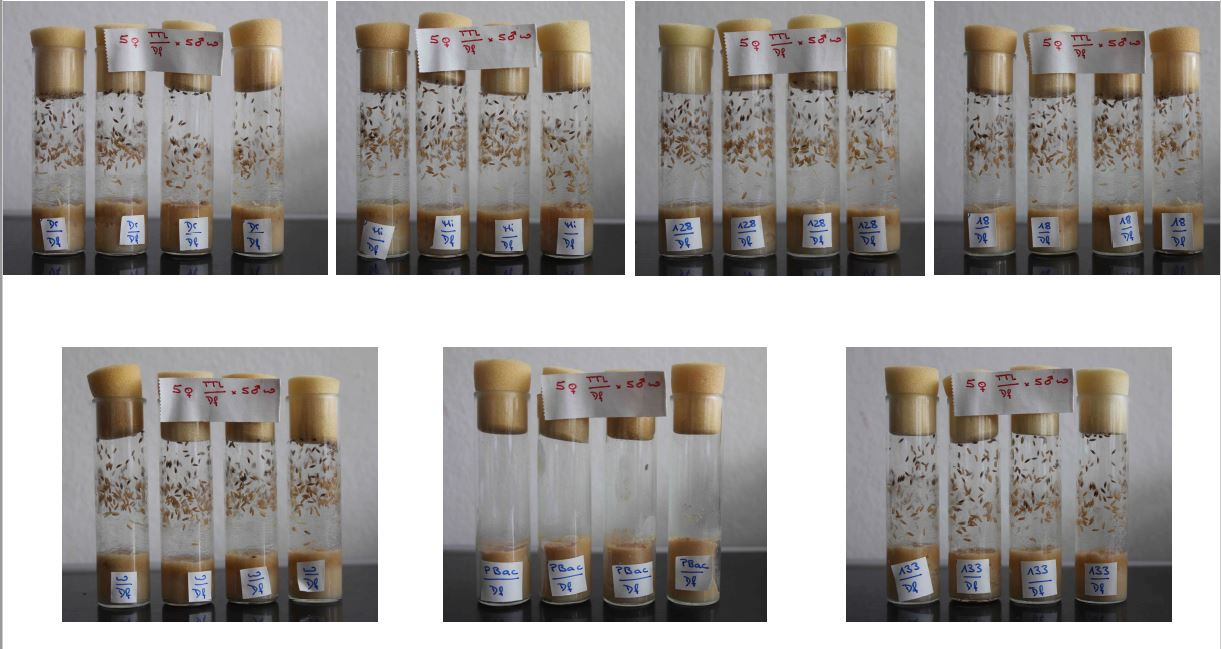
\includegraphics[width=1\linewidth]{img/fertility_test_results}
	\caption{}
	\label{fig:fertilitytestresults}
\end{figure}


% Please add the following required packages to your document preamble:
% \usepackage{graphicx}
\begin{table}[H]
	\centering
	\resizebox{\textwidth}{!}{%
		\begin{tabular}{|l|l|l|l|l|l|}
			\hline
			& Flies &  \begin{tabular}[c]{@{}l@{}}Hatching temp\\ of female\end{tabular} & Layed eggs & Unhatched eggs & Hatching rate \\ \hline
			4) &\T $w; \Tfrac{venus-TTLL}{venus-TTLL}; \Tfrac{venus-TTLL}{TM, Sb}$ \B & 25\degree C & 100 & 7 & 93 \\ \hline
			&\T  $w; \Tfrac{venus-TTLL}{Driver}; \Tfrac{venus-TTLL}{TM, Sb}$ \B & 25\degree C & 97 & 9 & 90.72 \\ \hline
			5) &\T  $w; \Tfrac{msps-mcherry}{msps-mcherry}$ \B & 25\degree C & 94 & 49 & 48 \\ \hline
			&\T  $w; \Tfrac{msps-mcherry}{TM, Sb}$ \B & 25\degree C & 100 & 48 & 52 \\ \hline
			&\T  $w;\Tfrac{Driver}{+} \Tfrac{msps-mcherry}{+}$ \B & 25\degree C & 100 & 67 & 33 \\ \hline
			&\T  $w;\Tfrac{Driver}{+} \Tfrac{msps-mcherry}{+}$ \B & 25\degree C & 9 & 4 & (56) \\ \hline
			6) &\T  $w;\Tfrac{TACC-mcherry}{TACC-mcherry}$ \B & 25\degree C & 91 & 29 & 68 \\ \hline
			&\T  $w;\Tfrac{TACC-mcherry}{TM, Sb}$ \B & 25\degree C & 88 & 66 & 25 \\ \hline
			&\T  $w; \Tfrac{Driver}{+}; \Tfrac{TACC-mcherry}{+}$ \B & 25\degree C & 111 & 79 & 29 \\ \hline
			2) &\T  $w; \Tfrac{venus-TTLL}{SM, Cy}; \Tfrac{Minos}{Df(TTLL)}$ \B & 29\degree C & 30 & 9 & 70 \\ \hline
			& \T $w; \Tfrac{venus-TTLL}{Driver}; \Tfrac{Minos}{Df(TTLL)}$ \B & 29\degree C & 73 & 6 & 92 \\ \hline
			4) &\T  $w; \Tfrac{venus-TTLL}{venus-TTLL}; \Tfrac{venus-TTLL}{TM, Sb}$ \B & 29\degree C & 86 & 17 & 80 \\ \hline
			&\T  $w; \Tfrac{venus-TTLL}{Driver}; \Tfrac{venus-TTLL}{TM, Sb}$ \B & 29\degree C & 85 & 14 & 84 \\ \hline
		\end{tabular}%
	}
\end{table}



%----------------------------------------------------------------------------------------
%	SECTION 3
%----------------------------------------------------------------------------------------
\newpage
\section*{Experiment 2: Ovary stainings of Staufen - Confocal microscopy}

\subsection*{Material and methods}

\textbf{Flies used for Western blot and ovary stainings:}\\
% $ \Tfrac{}{}; \Tfrac{}{} $

\begin{multicols}{2}
	\begin{Large}
		$\Tfrac{w}{w}; \Tfrac{Driver}{venus-TTLL}; \Tfrac{TTLL5^{PBac}}{Df(TTLL)} $\\
		
		$\Tfrac{w}{w}; \Tfrac{Driver}{venus-TTLL}; \Tfrac{TTLL5^{Minos}}{Df(TTLL)} $\\
		
		$\Tfrac{w}{w}; \Tfrac{Driver}{venus-TTLL}; \Tfrac{TTLL5^{Mi-Ex}}{Df(TTLL)} $\\
		
		$\Tfrac{w}{w}$\\
		
		$\Tfrac{w}{w}; \Tfrac{SM, Cy}{venus-TTLL | Driver}; \Tfrac{TTLL5^{PBac}}{Df(TTLL)} $\\
		
		$\Tfrac{w}{w}; \Tfrac{SM, Cy}{venus-TTLL | Driver}; \Tfrac{TTLL5^{Minos}}{Df(TTLL)} $\\
		
		$\Tfrac{w}{w}; \Tfrac{SM, Cy}{venus-TTLL | Driver}; \Tfrac{TTLL5^{Mi-Ex}}{Df(TTLL)} $\\
		
		$\Tfrac{w}{w}; \Tfrac{venus-TTLL}{Driver}; \Tfrac{venus-TTLL}{TM, Sb} $\\
		
		
	\end{Large}
\end{multicols}

\textbf{Crosses for Western blot and ovary staining:} \\

\begin{Large}
	1) $\Tfrac{w}{w}; \Tfrac{venus-TTLL}{(SM, Cy)}; \Tfrac{Df(TTLL)}{TM, Sb}$  x  $\Tfrac{w}{}; \Tfrac{Driver}{(SM, Cy)}; \Tfrac{TTLL5^{PBac}}{TM, Sb}$\\
	
	2) $\Tfrac{w}{w}; \Tfrac{venus-TTLL}{(SM, Cy)}; \Tfrac{Df(TTLL)}{TM, Sb}$  x  $\Tfrac{w}{}; \Tfrac{Driver}{(SM, Cy)}; \Tfrac{TTLL5^{Minos}}{TM, Sb}$\\
	
	3) $\Tfrac{w}{w}; \Tfrac{venus-TTLL}{(SM, Cy)}; \Tfrac{Df(TTLL)}{TM, Sb}$  x  $\Tfrac{w}{}; \Tfrac{Driver}{(SM, Cy)}; \Tfrac{TTLL5^{Mi-Ex}}{TM, Sb}$\\
	
	4) $\Tfrac{w}{w}; \Tfrac{Driver}{(SM, Cy)}; \Tfrac{Pr Dr}{TM, Sb}$  x  $\Tfrac{w}{}; \Tfrac{venus-TTLL}{(SM, Cy)}; \Tfrac{venus-TTLL}{TM, Sb}$\\
	
	$ \Tfrac{w}{w} $ 
	
	
\end{Large}


\newpage\textbf{Crosses offsprings and number of ovaries selected for Western and Confocal:}\\

% Please add the following required packages to your document preamble:
% \usepackage{graphicx}
\begin{table}[H]
	\centering
	\resizebox{0.7\textwidth}{!}{%
		\begin{tabular}{|l|l|l|l|}
			\hline
			& Flies & \begin{tabular}[c]{@{}l@{}}Confocal\\ Nb ovaries\end{tabular} & \begin{tabular}[c]{@{}l@{}}Western\\ Nb ovaries\end{tabular} \\ \hline
			1a &\T $ w; \Tfrac{Driver}{venus-TTLL}; \Tfrac{PBac}{Df}  $ \B & 2 & 8 \\ \hline
			1b &\T $ w; \Tfrac{Driver or venus}{SM Cy}; \Tfrac{PBac}{Df}  $ \B & 2 & 10 \\ \hline
			2a &\T $ w; \Tfrac{Driver}{venus-TTLL}; \Tfrac{Minos}{Df}  $ \B & 14 & 16 \\ \hline
			2b &\T $ w; \Tfrac{venus-TTLL}{SM Cy}; \Tfrac{Minos}{Df}  $ \B & $\sim$15 & 16 \\ \hline
			3a &\T $ w; \Tfrac{Driver}{venus-TTLL}; \Tfrac{Ex128}{Df}  $ \B & $\sim$16 & 21 \\ \hline
			3b &\T $ w; \Tfrac{Driver}{SM Cy}; \Tfrac{Ex128}{Df}  $ \B & $\sim$18 & 18 \\ \hline
			4a &\T $ w; \Tfrac{venus-TTLL}{Driver}; \Tfrac{venus-TTLL}{TM Sb}  $ \B & 16 & 16 \\ \hline
			4b &\T $ w; \Tfrac{venus-TTLL}{venus-TTLL}; \Tfrac{venus-TTLL}{TM Sb}  $ \B & $\sim$14 & 16 \\ \hline
			5 &\T $ w $ \B & 16 & 25 \\ \hline
		\end{tabular}%
	}
\end{table}

\newpage
\subsection*{Procedure}
\subsubsection*{Solutions}

\begin{enumerate}[leftmargin=4.5cm]
	\item [Antibodies: ] polyclonal rabbit antibody anti Staufen protein
	\item [] monoclonal mouse antibody anti GFP
	\item [] anti-mouse antibody, fluorophore coupled (Alexa Fluor 647)
	\item [] anti-rabbit antibody, fluorophore coupled (Alexa Fluor 488)
	\item [Hoechst] DNA coloration 
	\item [Rhodamine Phalloidin] Actin coloration
	\item [Ringer's] Isotonic solution containing \SI{6.5}{\gram} $NaCl$, \SI{0.42}{\gram} $KCl$, \SI{0.25}{\gram} $CaCl_2$ , \SI{0.2}{\gram} $NaHCO_3 $ in \SI{1}{\liter} $H_2O$. 
	\item [PFA]
	\item [Heptane]
	\item [DMSO]
	\item [PBS]
	\item [PBST]  PBS + 0.1\% Tween-20
	\item [Triton X-100]
	\item [Tween-20]
	\item [Milk powder (or BSA)]
	\item [Aquamount]
\end{enumerate}

\subsubsection*{Procedure}
To obtain nice ovaries, 3 days old females were kept with males on food containing dry yeast in non-crowding condition at 25\degree C. \\

\paragraph{Dissection and fixation}The ovaries were dissected in PBS and transfered in Eppendorf tubes (Eppendorf AG, Hamburg, Deutschland) containing : \SI{200}{\micro\liter} 4\%  PFA, \SI{600}{\micro\liter} Heptane and \SI{20}{\micro\liter}  DMSO. They were fixed during 20 minutes on a rotation wheel, rinsed 3 times with PBST and rehydrated in PBST during 20 minutes. Still in PBST, the ovaries were opened (not completely separate the ovarioles) and transferred in a \SI{500}{\micro\liter} reaction vial for blocking. 

\paragraph{Blocking} Ovaries were permeabilized and blocked for 45 minutes in PBS with 0.1\% Tween-20, 0.1\% Triton-X100 and 5\% milk powder. Then the blocking buffer has been carefully removed and the ovaries transferred into PCR tubes for primary antibody. To better see the ovaries to transfer, the blocking buffer can be diluted with PBST. 

\paragraph{Primary antibody} Ovaries were incubated overnight on a rotation wheel at 4\degree C in \SI{100}{\micro\liter} of primary antibody containing mouse anti-GFP (1:200) and rabit anti Staufen (1:200) in PBS with 0.1\% Tween-20 and 5\% milk powder. 

\paragraph{Secondary antibody} Ovaries were rinsed 3 times with PBST and washed 3 times in PBST during 20 minutes. They were then incubated 3 hours at room temperature on a rotation wheel in the dark in goat anti-mouse 647 (1:200) and goat anti-rabbit 488 (1:200) in PBS with 0.1\% Tween-20 and 5\% milk powder. 

\paragraph{Hoechst} Ovaries were rinsed 3 times with PBST and washed 3 times in PBST during 20 minutes. They were then incubated during 20 minutes in \SI{1}{\milli\liter} PBST, \SI{0.5}{\micro\liter} Hoechst 33528 to en end concentration of \SI{2.5}{\micro\liter}/\SI{}{\milli\liter}. At this stage, ovaries can be stored in the dark at 4\degree C during a couple of days before mounting.

\paragraph{Mounting} Ovaries were rinsed 3 times with PBST and washed 3 times in PBST during 20 minutes. To be mounted in Aquamount, ovaries were transfered onto labelled slides with a bit of PBST. Then, the ovarioles were separated before adding the Aquamout, covering with the coverslip and let settling before storage in the dark at 4\degree C.




\newpage
\subsection*{Results}

\begin{figure}[H]
	\centering
	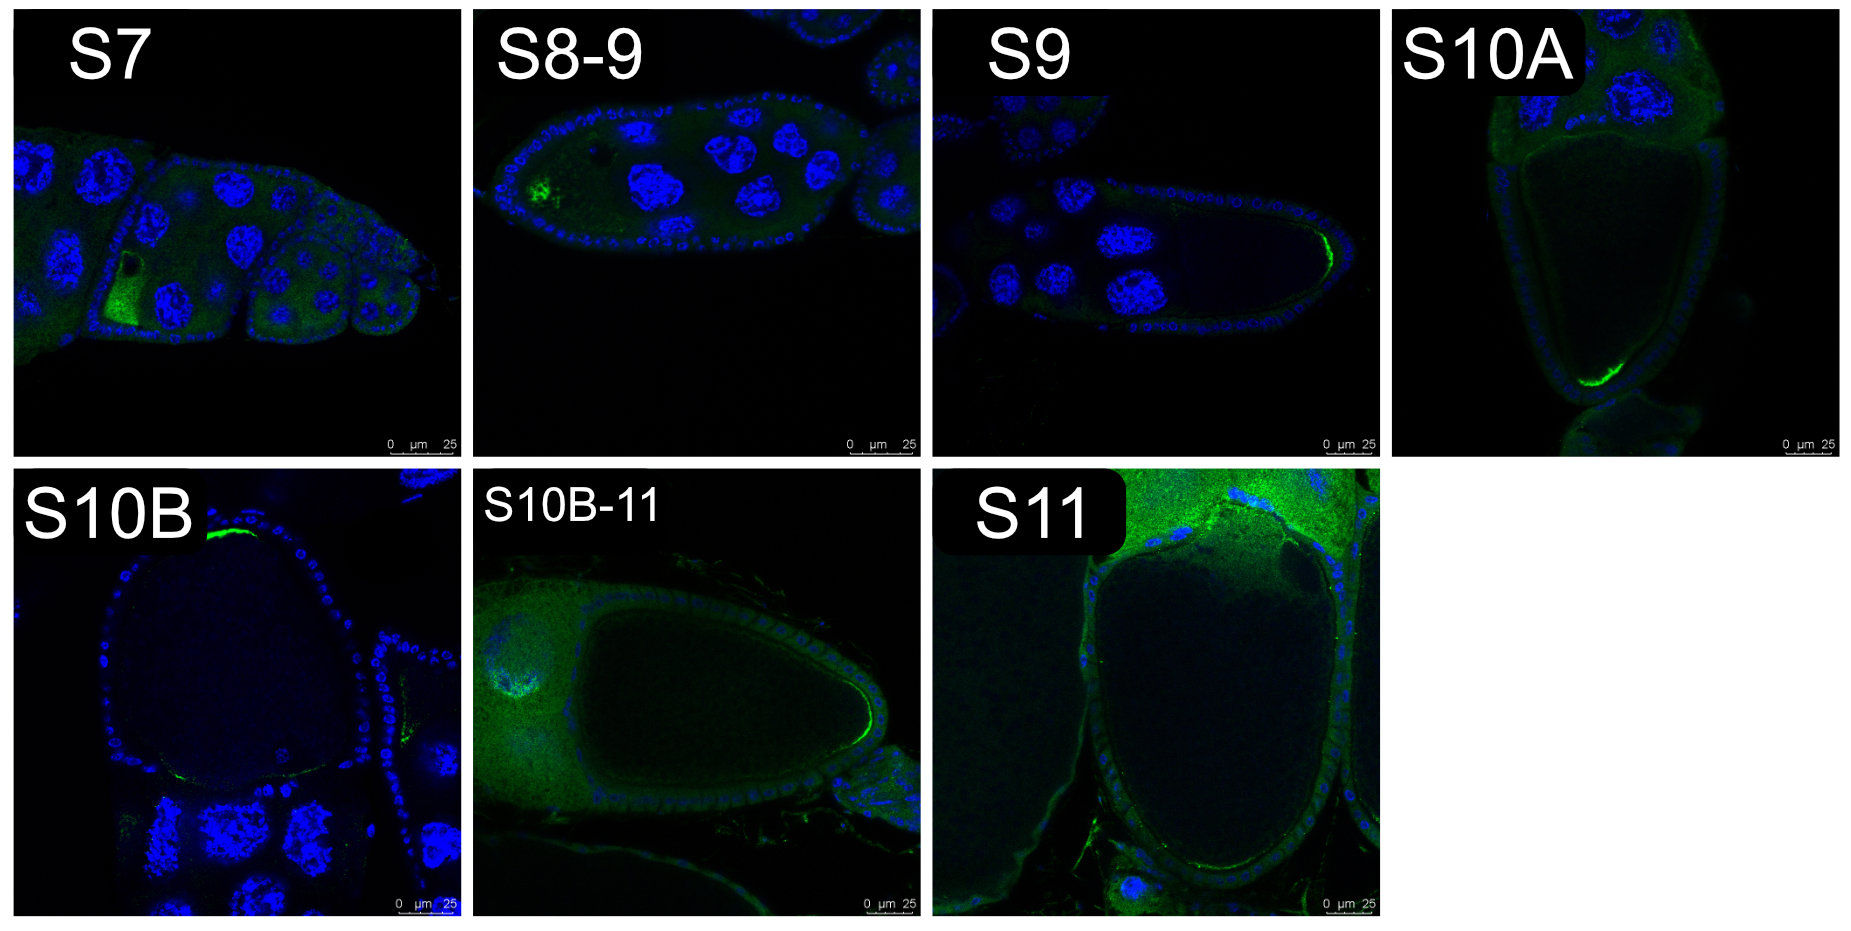
\includegraphics[width=0.9\linewidth]{img/confocal/confocal_white_hblock}
	\caption{White}
	\label{fig:confocalwhitehblock}
\end{figure}

\begin{figure}[H]
	\centering
	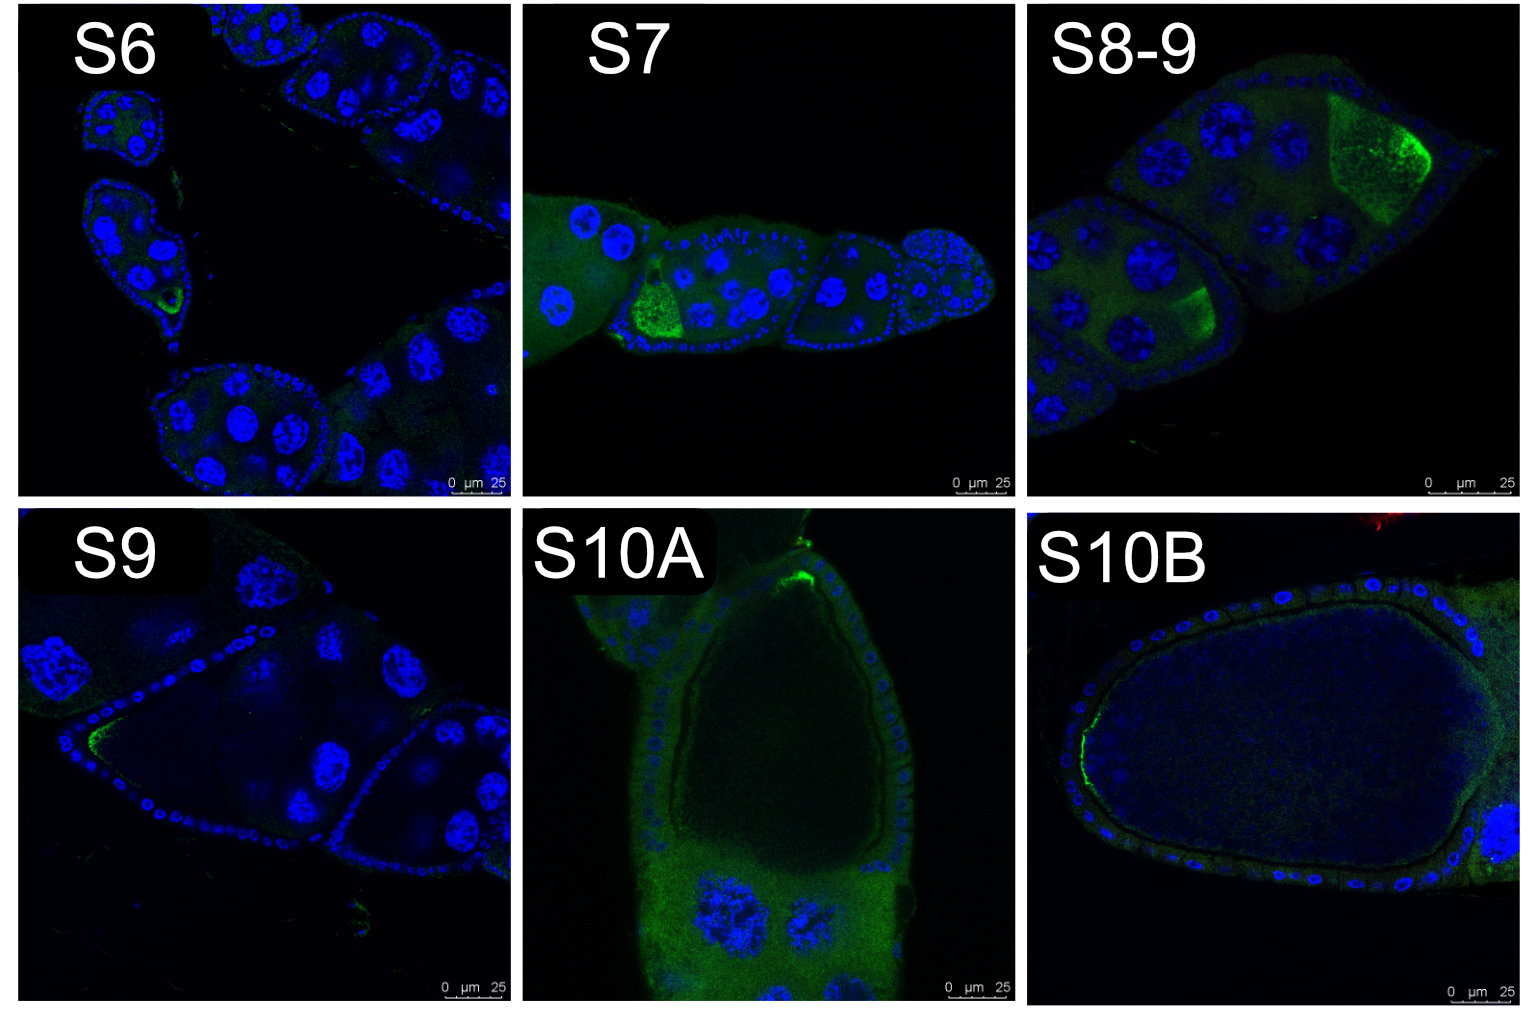
\includegraphics[width=0.9\linewidth]{img/confocal/confocal_ex128_Df_hblock}
	\caption{Ex128 over Df}
	\label{fig:confocalex128dfhblock}
\end{figure}

\begin{figure}[H]
	\centering
	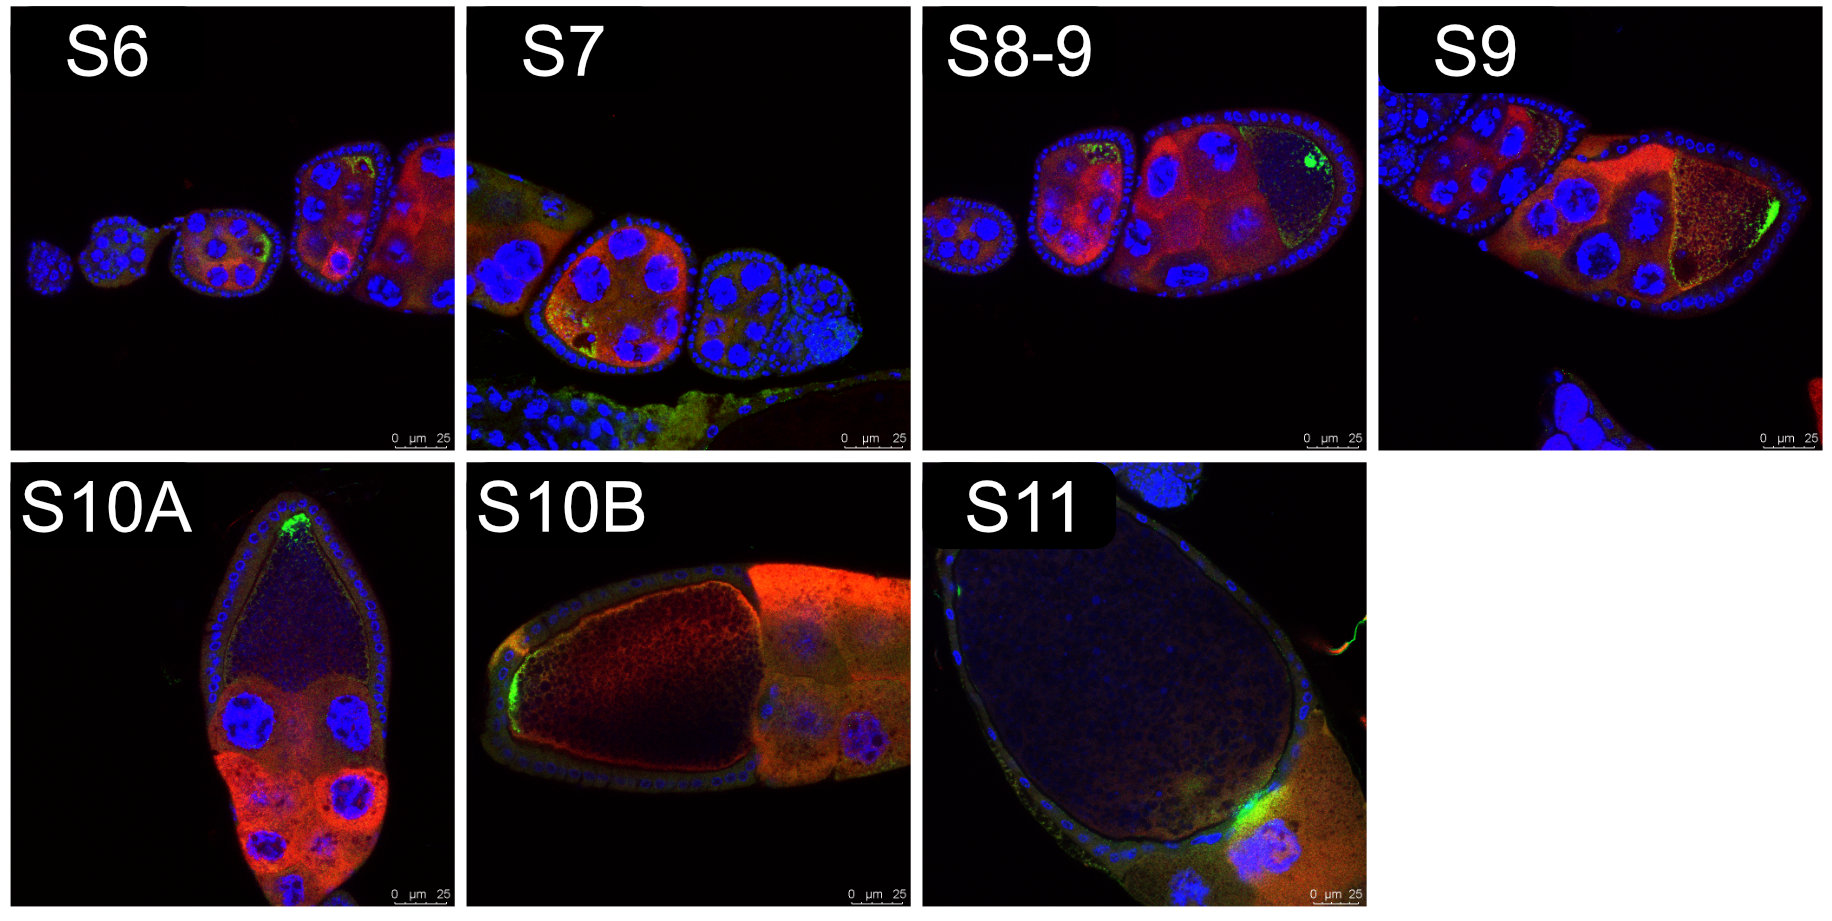
\includegraphics[width=0.9\linewidth]{img/confocal/confocal_ex128_Df_rescue_hblock}
	\caption{Ex128 over Df rescue}
	\label{fig:confocalex128dfrescuehblock}
\end{figure}





%----------------------------------------------------------------------------------------
%	SECTION 4
%----------------------------------------------------------------------------------------
\newpage
\section*{Experiment 3: Western blot}
\subsection*{Material and methods}
\textbf{Flies and ovaries number described in Experiment 2}.

%----------------------------------------------------------------------------------------
%	SECTION 5
%----------------------------------------------------------------------------------------
\newpage
\section*{Experiment 4: CRISPR/Cas9}


%----------------------------------------------------------------------------------------
%	SECTION 6
%----------------------------------------------------------------------------------------
\newpage
\section*{Conclusion and discussion}




%----------------------------------------------------------------------------------------
%	BIBLIOGRAPHY
%----------------------------------------------------------------------------------------

\bibliographystyle{apalike}

\bibliography{sample}

%----------------------------------------------------------------------------------------


\end{document}